\documentclass{article}
\usepackage{polski}
\usepackage{float}
\usepackage{amsmath, amssymb}
\usepackage{graphicx}
\usepackage{tikz}
\usepackage{geometry}
\graphicspath{ {./plots/} }

\title{Sprawozdanie 4 - Algorytmy Optymalizacji Dyskretnej}
\author{Michał Kallas}

\setlength\parindent{0pt}

\begin{document}

\maketitle

\section{Zadanie 1}
\subsection{Opis zadania}
Zadanie polega na napisaniu programu do obliczania maksymalnego przepływu w skierowanym grafie o strukturze hiperkostki $H_k$ za pomocą algorytmu Edmondsa-Karpa.
Należy przeprowadzić eksperymenty sprawdzające działanie algorytmu dla różnych rozmiarów hiperkostki.

\subsection{Opis grafu}
Rozważany w tym zadaniu graf to hiperkostka $H_k$.
Jest to graf skierowany o $2^k$ wierzchołkach.
Wierzchołki hiperkostki odpowiadają k-bitowym ciągom binarnym, a krawędzie łączą wierzchołki różniące się na dokładnie jednej pozycji bitowej.
Pojemności krawędzi są losowane niezależnie z rozkładem jednostajnym ze zbioru $\{1, \dots, 2^l\}$, gdzie $l = \max\{H(e(i)), Z(e(i)), H(e(j)), Z(e(j))\}$.
$H(x)$ to waga Hamminga, czyli ilość jedynek w ciągu bitowym $x$, a $Z(x)$ to ilość zer w $x$.
Dla ciągu długości $k$ $H(X)$ oraz $Z(x)$ przyjmują wartości ze zbioru $\{0, 1, \dots, k\}$.

\subsection{Opis algorytmu}
Do obliczenia maksymalnego przepływu zastosowano algorytm Edmondsa-Karpa, będący implementacją metody Forda-Fulkersona.
Graf, na którym będzie pracował algorytm, to graf residualny, czyli taki, który dla każdej krawędzi posiada dodatkową krawędź w kierunku przeciwnym do kierunku przepływu(aby móc odrzucać niewłaściwe ścieżki powiększające).
Każda krawędź ma pewną nieujemną pojemność oraz wartość przepływu, która początkowo wynosi zero.
Algorytm działa w następujący sposób:
\begin{enumerate}
\item Inicjalizuj wartość maksymalnego przepływu na 0.
\item Wykorzystaj BFS do znalezienia najkrótszej ścieżki z wierzchołka źródłowego $s$ do ujścia $t$.
\item Jeśli taka ścieżka nie istnieje, zakończ algorytm.
\item Wylicz maksymalny przepływ dla tej ścieżki, czyli minimum z aktualnej pojemności krawędzi (pojemność krawędzi krytycznej) na tej ścieżce - $c_{min}$.
\item Zaktualizuj przepływ wzdłuż tej ścieżki o $c_{min}$, zwiększając przepływy na krawędziach w kierunku przepływu i zmiejszając przepływy w przeciwnym kierunku.
\item Zaktualizuj wartość maksymalnego przepływu o $c_{min}$.
\item Powtarzaj kroki 1-6.\\
\end{enumerate}

Złożoność algorytmu Edmondsa-Karpa wynosi $O(|V||E|^2)$, dlatego że koszt BFSa to $O(|E|)$ na iterację, a wybierając najkrótsze ścieżki powiększające, musimy wykonać $O(|V||E|)$ powiększeń przepłwu.\\

Algorytm zaimplementowałem w języku C++.

\subsection{Opis eksperymentu}
Eksperyment polegał na sprawdzeniu zachowania algorytmu Edmondsa-Karpa dla hiperkostek $H_k$, $k \in \{1, 2, \dots, 16\}$.
Zostały sprawdzone 3 kryteria:
\begin{itemize}
\item Średni czas działania algorytmu
\item Średni wyliczony maksymalny przepływ
\item Średnia wyliczona ilość ścieżek powiększających
\end{itemize}
Dla każdego $k$ eksperyment był przeprowadzony na 100 losowych hiperkostkach.

\subsection{Wyniki eksperymentu}
\begin{figure}[H]
\centering
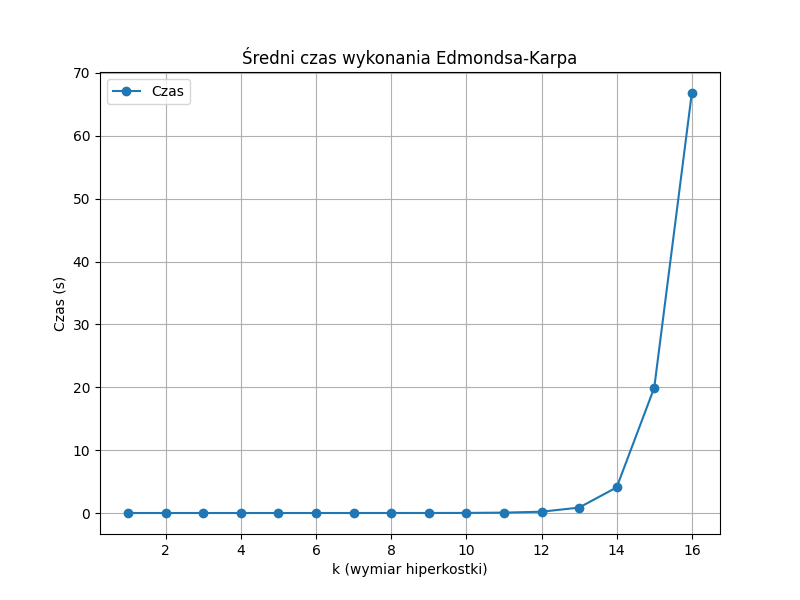
\includegraphics[width=0.67\textwidth]{edmondsKarpTimePlot.png}
\caption{Uśredniony czas wykonania algorytmu Edmondsa-Karpa w sekundach.}
\end{figure}

\begin{figure}[H]
\centering
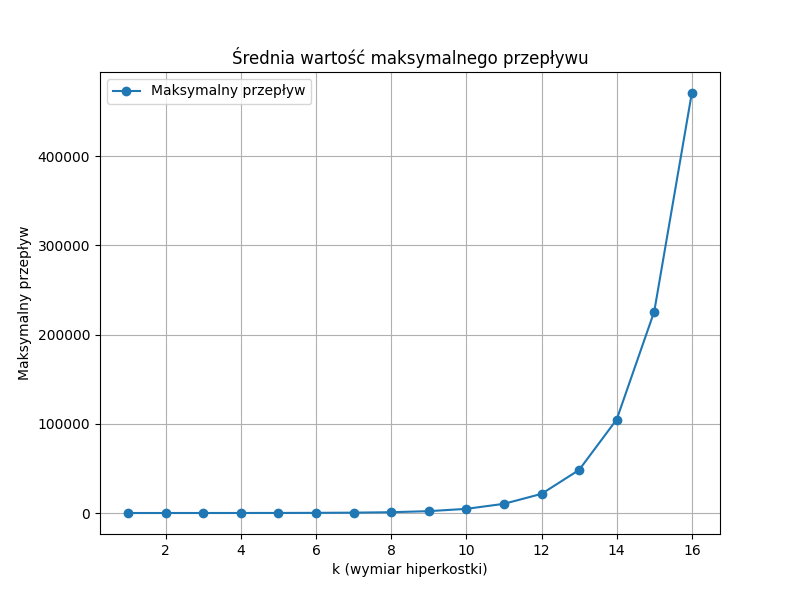
\includegraphics[width=0.67\textwidth]{edmondsKarpFlowPlot.png}
\caption{Średni wyliczony maksymalny przepływ przez algorytm Edmondsa-Karpa.}
\end{figure}

\begin{figure}[H]
\centering
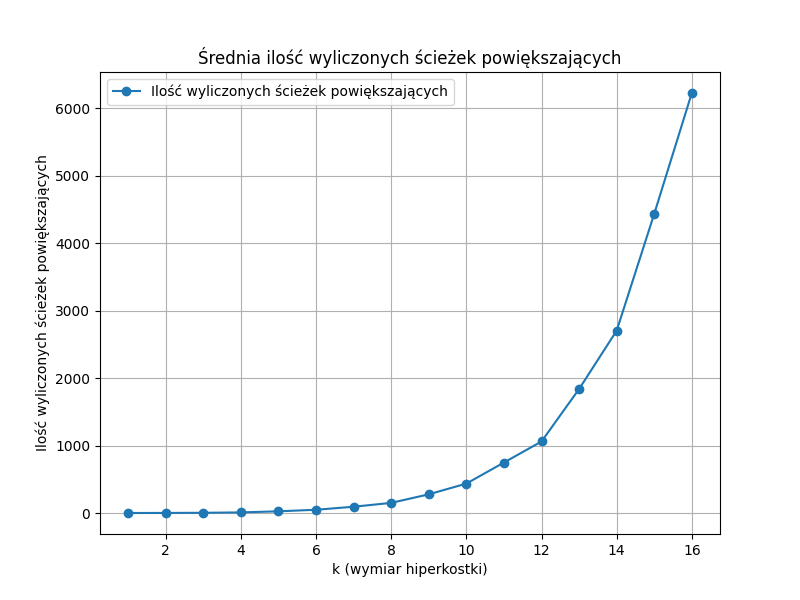
\includegraphics[width=0.67\textwidth]{edmondsKarpPathPlot.png}
\caption{Średnia ilość wyliczonych ścieżek powiększających przez algorytm Edmondsa-Karpa.}
\end{figure}

\subsection{Wyniki eksperymentu}
Na wykresie prezentującym średnie czasy widać, że algorytm Edmondsa-Karpa dobrze radzi sobie dla mniejszych hiperkostek, ale dla $k \ge 14$ czas zaczyna gwałtownie rosnąć.
Taki stan rzeczy jest spodowany tym, że wielkości hieperkostek rosną wykładniczo, jako że ich ilość wierzchołków to $2^k$, a ilość krawędzi $2^{k - 1} \cdot k$.
Złożoność algorytmu wynosi $O(|V||E|^2)$, a więc jest ona w tym przypadku wykładniczo zależna od $k$.
Widać, że średnia wartość maksymalnego przepływu i ilość wyliczonych ścieżek powiększających także zależą wykładniczo od $k$.\\

Możemy wnioskować, że algorytm Edmondsa-Karpa będzie odpowiedni do liczenia przepływów w mniejszych hiperkostkach.
Dla większych $H_k$ jest on za wolny ze względu na złożoność wykładniczą.

\section{Zadanie 2}
\subsection{Opis zadania}
Zadanie polega na napisaniu programu do wyliczenia wielkości skojarzenia o największym rozmiarze dla grafu dwudzielnego.
Tutaj także należy eksperymentalnie sprawdzić działanie programu.

\subsection{Opis grafu}
Rozważany w tym zadaniu graf to nieskierowany dwudzielny graf losowy, mający dwa rozłączne podzbiory wierzchołków $V_1$, $V_2$, każdy o mocy $2^k$, gdzie $k \in \mathbb{N}$.
Każdy z wierzchołków tego grafu ma stopień wynoszący $i$, gdzie $i \in \mathbb{N}$.

\subsection{Przekształcenie problemu}
Do rozwiązania problemu wyliczenia wielkości skojarzenia o największym rozmiarze możemy ponownie skorzystać z algorytmu Edmondsa-Karpa.
Jednak, aby tego dokonać, musimy w pierwszej kolejności przekształcić problem do problemu wyznaczenia maksymalnego przepływu.

Aby przekształcić problem, musimy zamienić nasz nieskierowany graf dwudzielny w graf skierowany, łączący wierzchołki z $V_1$ do $V_2$ krawędziami o pojemności 1.
Potrzebne są nam także źródło $s$ oraz ujście $t$.
Wierzchołek $s$ połączymy z każdym wierzchołkiem ze zbioru $V_1$, a każdy wierzchołek ze zbioru $V_2$ połączymy z wierzchołkiem $t$.
Pojemności tych krawędzi także będą wynosiły 1.
Takie przekształcenie wygląda następująco:

\begin{center}
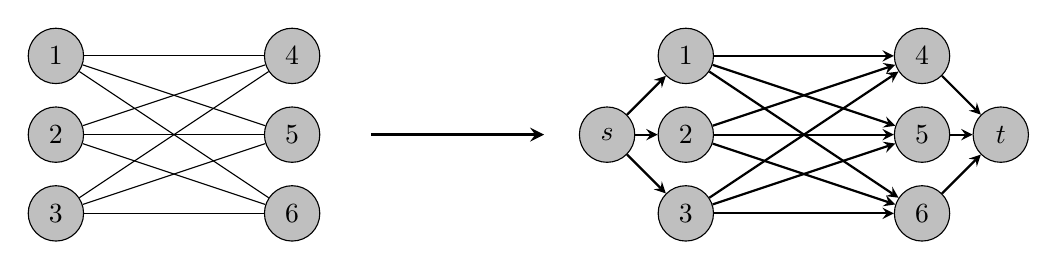
\begin{tikzpicture}
    \tikzstyle{vertex}=[circle, draw, fill=black!25, minimum size=20pt, inner sep=0pt]

    \foreach \i in {1, 2, 3}
        \node[vertex] (L\i) at (0, -\i) {$\i$};
    \foreach \i in {4, 5, 6}
        \node[vertex] (R\i) at (3, -\i+3) {$\i$};

    \foreach \i in {1, 2, 3}
        \foreach \j in {4, 5, 6}
            \draw (L\i) -- (R\j);

    \foreach \i in {1, 2, 3}
        \node[vertex] (L2\i) at (8, -\i) {$\i$};
    \foreach \i in {4, 5, 6}
        \node[vertex] (R2\i) at (11, -\i+3) {$\i$};

    \node[vertex] (S) at (7, -2) {$s$};
    \node[vertex] (T) at (12, -2) {$t$};

    \foreach \i in {1, 2, 3}
        \foreach \j in {4, 5, 6}
            \draw[->, thick, >=stealth] (L2\i) -- (R2\j);

    \foreach \i in {1, 2, 3}
        \draw[->, thick, >=stealth] (S) -- (L2\i);
    \foreach \i in {4, 5, 6}
        \draw[->, thick, >=stealth] (R2\i) -- (T);

    \draw[->, very thick, >=stealth] (4, -2) -- (6.2, -2);
\end{tikzpicture}
\end{center}

\subsection{Opis eksperymentu}
Eksperyment polegał na sprawdzeniu średniego czasu wykonania programu oraz średniej wielkości maksymalnego skojarzenia dla $k \in \{3, \dots, 10\}$ oraz $i \in \{1, \dots, k\}$.
Dla każdego $k$ należało wygenerować wykres wielkości maksymalnego skojarzenia w zależności od $i$, a dla każdego $i$ wykres czasu działania programu w zależności od $k$.
Dla każdej pary $(k, i)$ eksperyment był przeprowadzony na 1000 losowych grafów.

\subsection{Wyniki eksperymentu}
\begin{figure}[H]
\centering
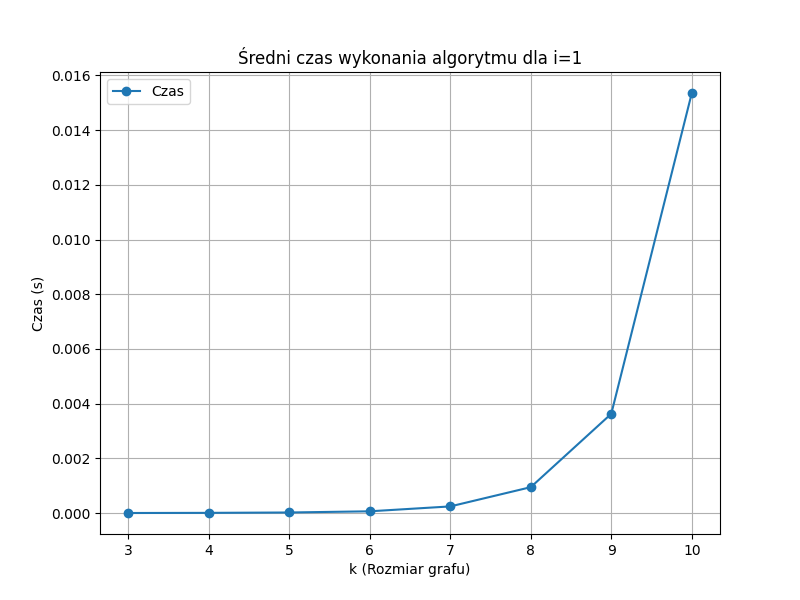
\includegraphics[width=0.46\textwidth]{maximumBipartiteMatchingTimePlot1.png}
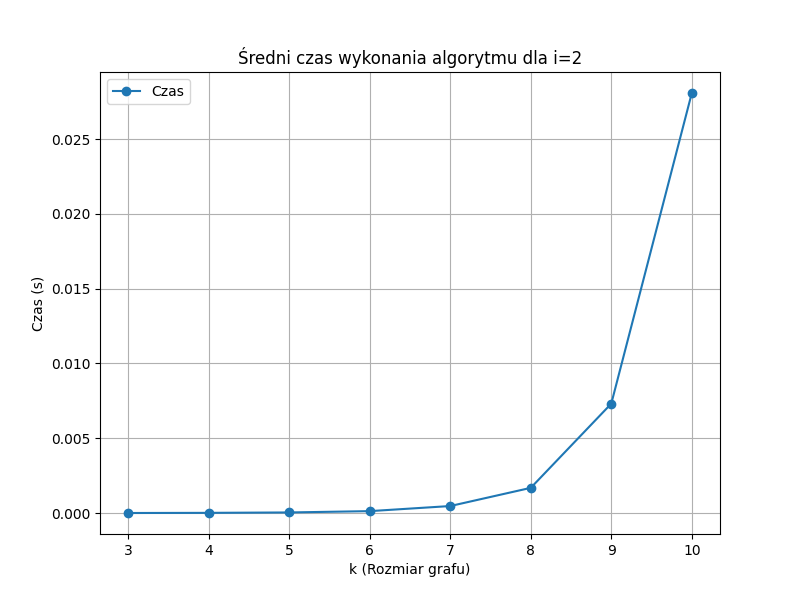
\includegraphics[width=0.46\textwidth]{maximumBipartiteMatchingTimePlot2.png}
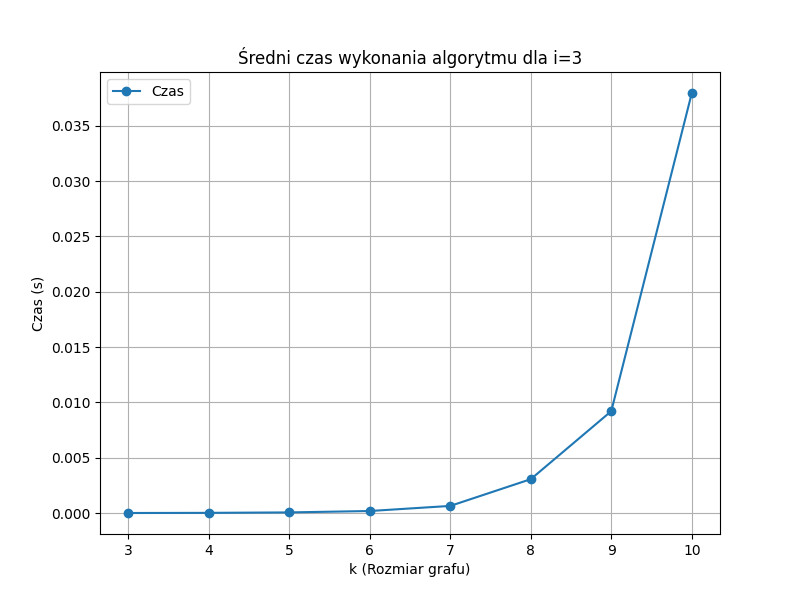
\includegraphics[width=0.46\textwidth]{maximumBipartiteMatchingTimePlot3.png}
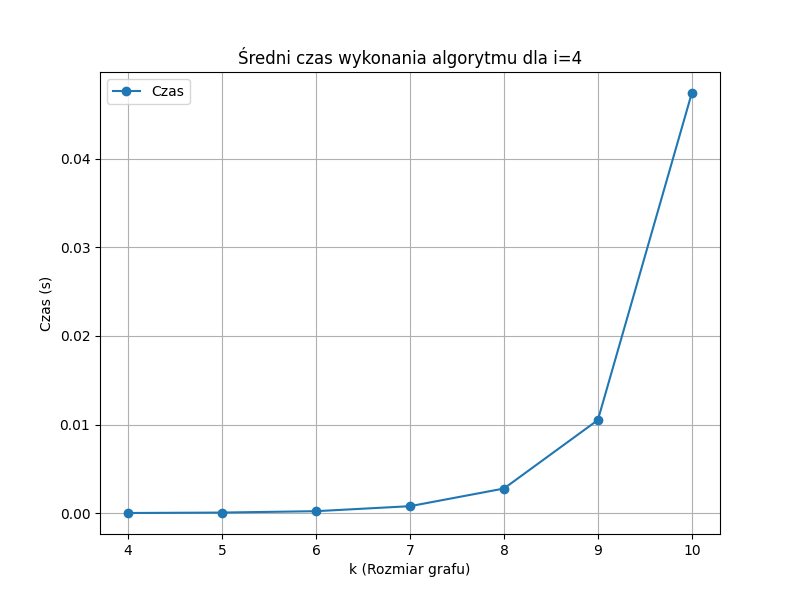
\includegraphics[width=0.46\textwidth]{maximumBipartiteMatchingTimePlot4.png}
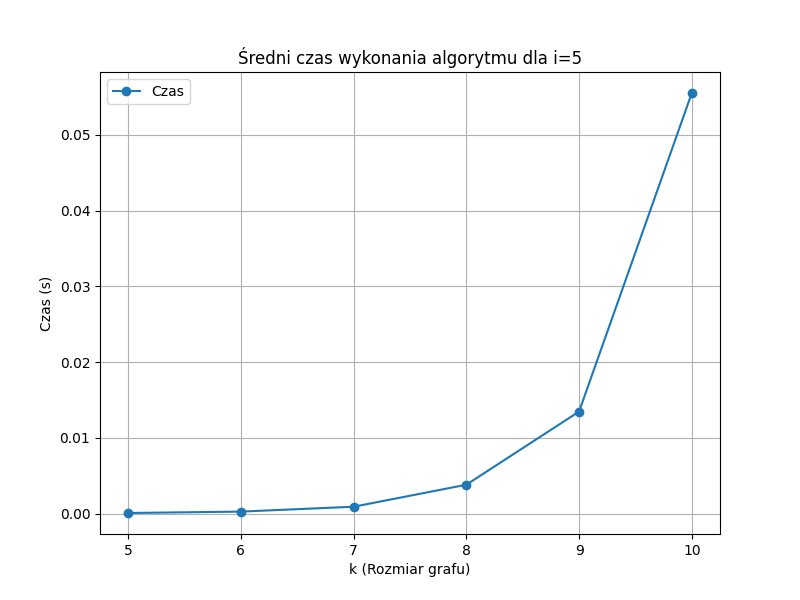
\includegraphics[width=0.46\textwidth]{maximumBipartiteMatchingTimePlot5.png}
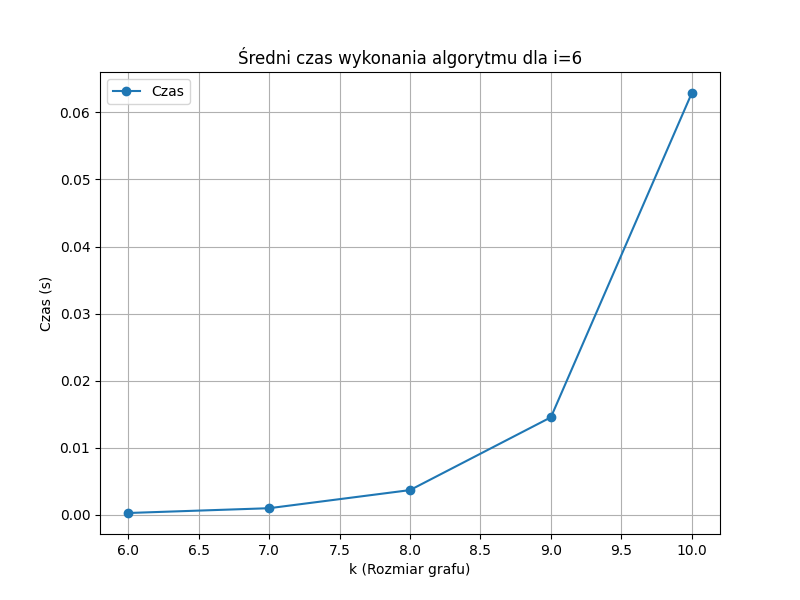
\includegraphics[width=0.46\textwidth]{maximumBipartiteMatchingTimePlot6.png}
\caption{Uśredniony czas wykonania algorytmu Edmondsa-Karpa w sekundach dla problemu wyliczenia wielkości skojarzenia o największym rozmiarze.}
\end{figure}

\begin{figure}[H]
\centering
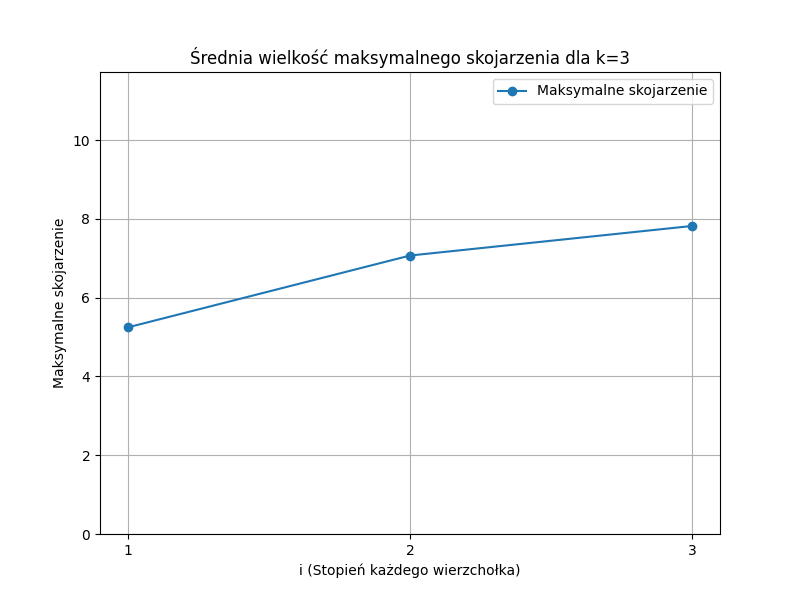
\includegraphics[width=0.46\textwidth]{maximumBipartiteMatchingMaxMatchingPlot3.png}
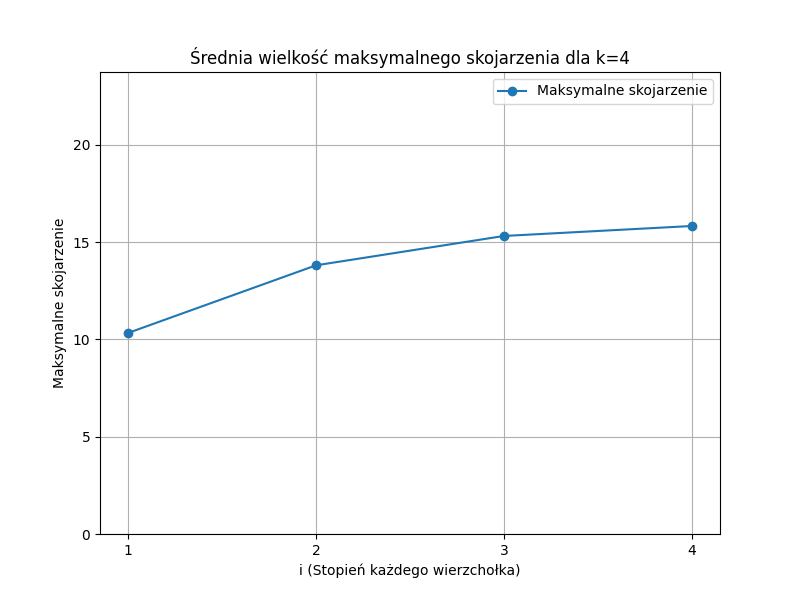
\includegraphics[width=0.46\textwidth]{maximumBipartiteMatchingMaxMatchingPlot4.png}
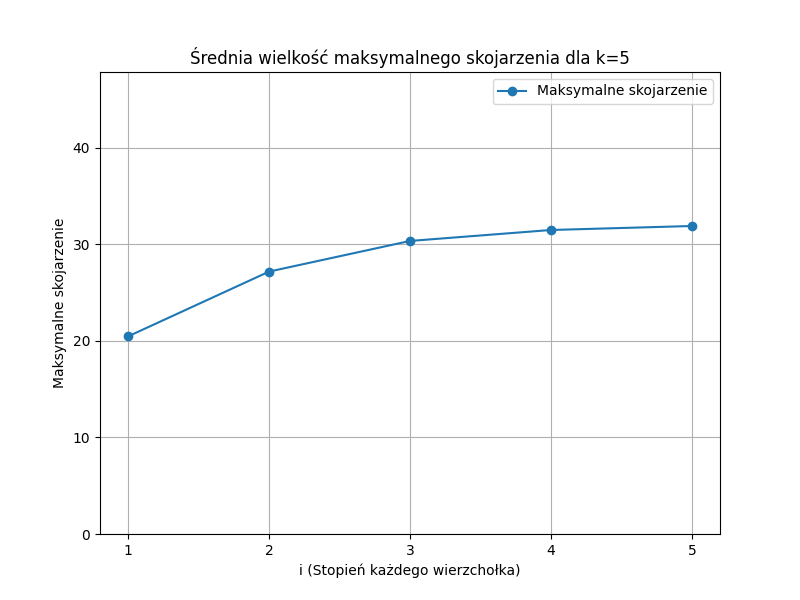
\includegraphics[width=0.46\textwidth]{maximumBipartiteMatchingMaxMatchingPlot5.png}
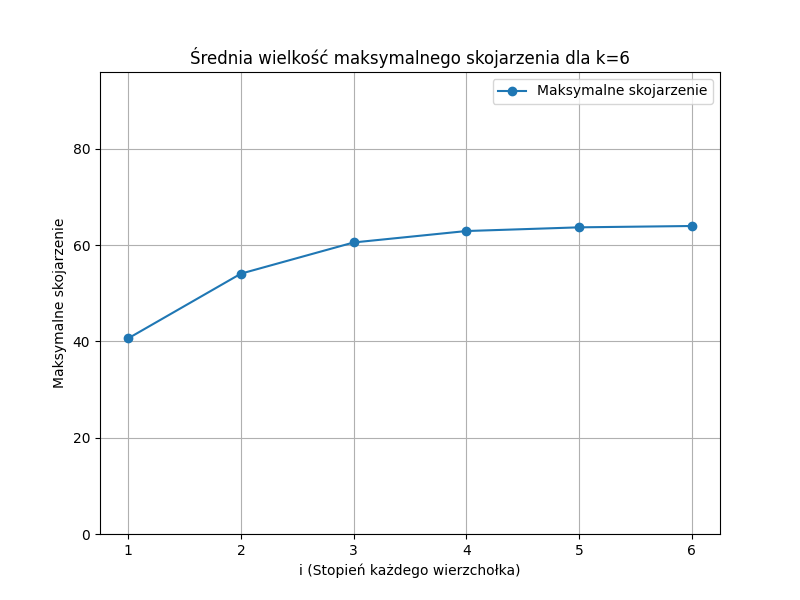
\includegraphics[width=0.46\textwidth]{maximumBipartiteMatchingMaxMatchingPlot6.png}
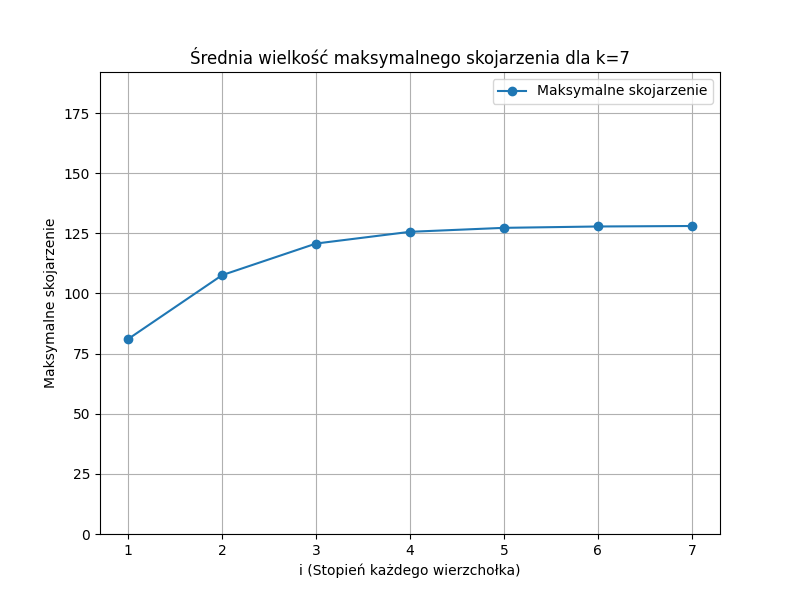
\includegraphics[width=0.46\textwidth]{maximumBipartiteMatchingMaxMatchingPlot7.png}
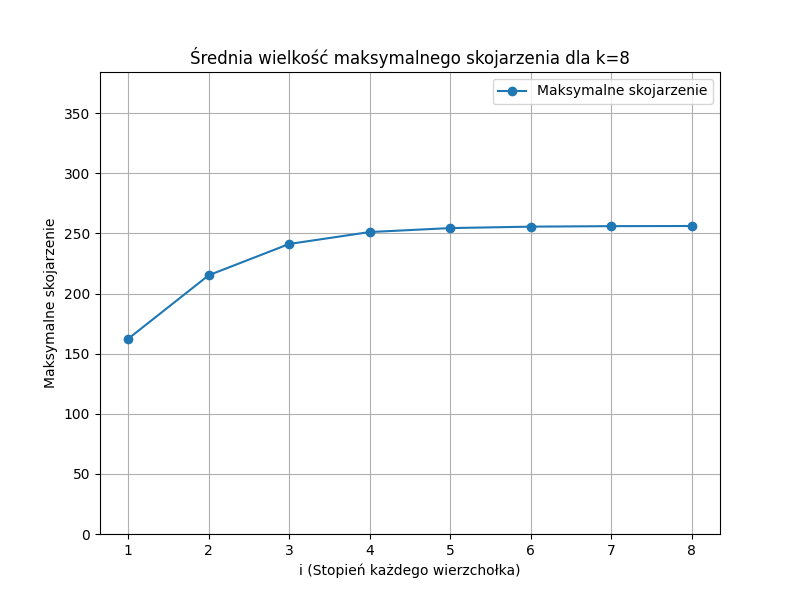
\includegraphics[width=0.46\textwidth]{maximumBipartiteMatchingMaxMatchingPlot8.png}
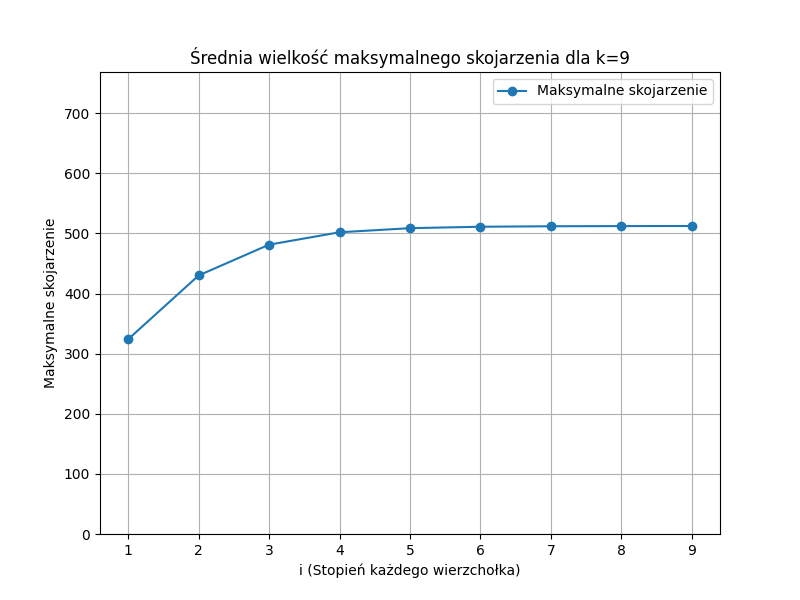
\includegraphics[width=0.46\textwidth]{maximumBipartiteMatchingMaxMatchingPlot9.png}
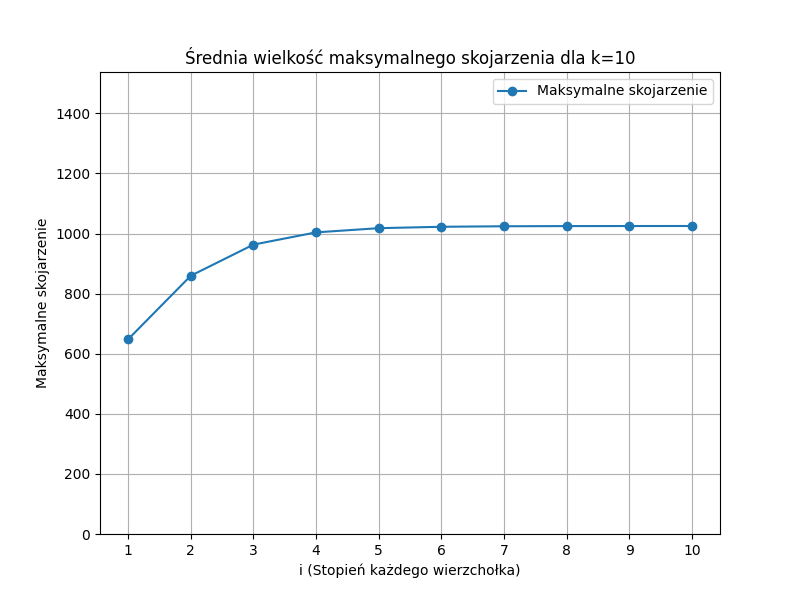
\includegraphics[width=0.46\textwidth]{maximumBipartiteMatchingMaxMatchingPlot10.png}
\caption{Średnia wielkość maksymalnego skojarzenia wyliczona przez algorytmu Edmondsa-Karpa.}
\end{figure}

\subsection{Obserwacje i wnioski}
Możemy zauważyć, że czas wykonania programu rośnie wykładniczo wraz ze wzrostem $k$, a $i$ także wpływa na jego wzrost.
Złożoność algorytmu Edmondsa-Karpa, wynosząca $O(|V||E|^2)$, ponownie tłumaczy nam skąd wziął się taki stan rzeczy.
W rozważanym grafie ilość wierzchołków to $2^{k + 1} + 2$, a ilość krawędzi to $(i + 2) \cdot 2^k$.\\

Dla rozważanego grafu średnia wielkość maksymalnego skojarzenia jest duża dla każdych rozważanych danych - wszędzie już dla $i=1$ jest ponad połową maksymalnej wartości.
Zbiega do $2^k$, czyli największego możliwego skojarzenia do uzyskania (bo w każdym zbiorze grafu dwudzielnego jest $2^k$ wierzchołków).
Dla $k = i$ te wartości w każdym przypadku są praktycznie równe.

\section{Zadanie 3}
\subsection{Opis zadania}
W tym zadaniu należy ponownie rozwiązać problemy maksymalnego przepływu oraz maksymalnego skojarzenia dla takich samych grafów, ale tym razem należy to zrobić poprzez wygenerowanie modeli programowania liniowego i skorzystanie z solvera \texttt{glpk} do ich rozwiązania.

\subsection{Opis modelu}
Program generujący pliki z modelami programowania liniowego napisałem w C++. Pliki wynikowe są napisane w Julii. Do pisania modeli wykorzystałem biblioteki \texttt{JuMP} i \texttt{GLPK}.\\

W generowanym pliku z modelem jest tworzona macierz rozmiaru $n \times n$ reprezentująca dany graf.
Zmienną decyzyjną służącą do przechowywania przepływów jest $f_{ij} \ge 0$. W $f_{ij}$ przechowywany jest przepływ z wierzchołka $i$ do wierzchołka $j$.\\

Zostały zastosowane następujące ograniczenia:
\begin{itemize}
    \item Przepływy muszą być nie większe od pojemności:
    $$
    f_{ij} \le u_{ij}
    $$
    \item Przepływy muszą być zbalansowane:
    $$
    \sum_{j=1}^n f_{i,j} = \sum_{j=1}^n f_{j,i} \quad \forall i \in \{2, \ldots, n-1\}
    $$
\end{itemize}

Celem była maksymalizacja przepływów:
$$
\max \sum_{j=1}^n f_{1,j}
$$

\subsection{Obserwacje i wnioski}
Solver zwraca takie same wartości maksymalnych przepływów i skojarzeń, jak algorytm Edmondsa-Karpa.
Jednakże dochodzi do tych wyników w inny sposób - wartości poszczególnych przepływów i skojrzeń różnią się od tych wyliczonych przez algorytm Edmondsa-Karpa.
Niestety solver czasami nie jest w stanie wyznaczyć rozwiązania ze względu na zbyt mało dostępnej pamięci.\\

Jeśli chodzi o prędkość działania, to tutaj solver wypada fatalnie.
Jest o rzędy wartości wolniejszy.
Przykładowo dla hiperkostki $H_7$, Edmonds-Karp poradził sobie z problemem w 6ms, podczas gdy solverowi zajęło to prawie 4 sekundy.\\


Okazuje się, że algorytm Edmondsa-Karpa jest znacznie lepszym rozwiązaniem problemów przedstawionych na tej liście niż programowanie liniowe.
Pomimo wykładniczych czasów działania wciąż jest nieporównywalnie szybszy. Co więcej, nie ma problemów z pamięcią.


\end{document}
